% Print
\documentclass[headinclude=true]{scrartcl}

%Packages, die für die deutsche Sprache erforderlich sind
\usepackage[utf8]{inputenc}
\usepackage[T1]{fontenc}
\usepackage{lmodern}
\usepackage[ngerman]{babel}
\usepackage{csquotes}

%Packages für Graphik
\usepackage[]{graphicx}
\graphicspath{{figures/}}

%BibLaTex
\usepackage[backend=biber]{biblatex}
\addbibresource{literature/bibliography.bib} 

%Package, damit Bibtex-URL klappt
\usepackage[pdfusetitle]{hyperref}
\usepackage{url}

%Noch schönere Typographie
\usepackage{microtype}

\usepackage{todonotes}

%Kästen
\usepackage{framed}

%%%%% BEGINN KOPF- UND FUẞZEILE %%%%%
\usepackage[headsepline,footsepline]{scrlayer-scrpage}
\usepackage{graphicx}
\pagestyle{scrheadings}
\ohead{\includegraphics[height=1cm]{figures/bluemarble}}
\chead{\headmark}
\automark{section}
%\ihead{\includegraphics[height=1cm]{bluemarble.jpg}}
\ifoot{\csname @title\endcsname}\cfoot{\pagemark}
\ofoot{\today}
%%%%% ENDE KOPF- UND FUẞZEILE %%%%%

\begin{document}
%%%%% BEGINN TITEL %%%%%
\title{Projektaufgabe}
\subtitle{Entwicklungsmethoden für nachhaltige Produkte}
\author{EnWiNaP-Team}
\maketitle
%%%%% ENDE TITEL %%%%%

%%%%% BEGINN FRONT MATTER %%%%%
\tableofcontents
%%%%% ENDE FRONT MATTER %%%%%


%%%%% BEGINN INHALT %%%%%


\section{Einleitung}

Viele Produkte die wir im Alltag nutzen, haben teils gravierende ökologische und/oder soziale Auswirkungen. 
Sie werden aus Rohstoffen und Materialien hergestellt, die in ihrer Herstellung Umweltschäden hervorrufen oder unter menschenunwürdigen Bedingungen abgebaut werden (z.B. Tantal für Mikroelektronik \cite{Schippers.2020}). Viele Inhaltsstoffe können darüber hinaus eine Gefahr für die Gesundheit der Nutzenden bedeuten (z.B. Inhaltsstoffe in Plastik \cite{BUND.2021}).
Das Design vieler Produkte ist auf eine kurze Nutzungsdauer ausgerichtet und erschwert oder verhindert ein Reparieren häufig auftretender Mängel zugusten von schnelleren und günstigeren Produktionsprozessen (z.B. verklebte Handydisplays). Diese Problematik wird durch den Trend verstärkt, dass immer mehr Produkte auf regelmäßige Softwareupdatens angewiesen sind.
So kann ein voll funktionsfähiges Smart-TV nutzlos werden, wenn das Modell für die neusten Softwareversionen nicht mehr unterstützt wird.
Ein weiteres Problem ist die Schwierigkeit, die Materialien in heutigen Produkte zu einem akzeptablen Grad zu recyceln. Und nicht zuletzt geht die Produktion vieler Produkte mit einer Ausbeutung der Produzierenden einher \cite{Kollross.2017}.

Da es außer dem Energielabel für Elektrogeräte keine verpflichtenden Ratings für die Nachhaltigkeit von Produkten gibt, ist es für die Endkund*innen sehr schwer einzuschätzen, wie schädlich das gekaufte Produkt wirklich ist. Und selbst verlässliche Studien, die die Auswirkungen der Produkte konkurrierender Hersteller vergleichen, sind nicht ohne weiteres zu finden, sodass der Wunsch nachhaltigere Produkte zu kaufen für die Mehrzahl der Nutzer*innen schwer umsetzbar ist.

Für einige Produkte gibt es bereits gute Ansätze, die negativen Auswirkungen zu minimieren. Beispiel sind hier z.B. faire und ökologische Kleidung und auf Nachhaltigkeit hin optimierte Smartphones wie Shift\footnote{\url{www.shiftphones.com}} oder Fairphone\footnote{\url{www.fairphone.com/de}}. Doch auch solche Produkte können über Rebound-Effekte unter dem Strich wieder eine negative Bilanz aufweisen da sie den Kund*innen vermitteln, hier mit gutem Gewissen konsumieren zu können und so zu noch mehr Konsum anregen.
So stellt sich die Frage, ob die reine Verringerung der negativen Auswirkungen von Produkten überhaupt einen positiven Effekt haben kann \cite{Carstens.2018, Braungart.2013}.
Endverbraucher*innen bleibt zwar die Möglichkeit, second-hand oder überarbeitete Produkte zu kaufen um ihren negativen Einfluss zu reduzieren. Doch für die überwiegende Mehrzahl von alltäglich genutzten Produkten suchen wir bei der Neubeschaffung heute noch vergeblich nach nachhaltigen Alternativen.

Das sollte sich ändern!

\subsection{Die Aufgabe}

Die oben vorgestellte Problemstellung hat euch dazu bewegt, aktiv zu werden. Als junge Ingenieur*innen seht ihr hier eine Herausforderung, der ihr euch gerne stellen möchtet. 
Ihr habt (natürlich) direkt eine Idee im Kopf, welches Produkt unbedingt nachhaltiger gestaltet werden müsste. Eure Aufgabe in diesem Semester ist es nun, euch der Verbesserung dieses Produktes methodisch zu nähern. 

Als ersten Schritt wollt ihr eine grundsätzliche Analyse des Sachverhaltes liefern. Diese soll den ist-Zustand des Produktes beleuchten und mithilfe bestehender Studien dessen Probleme herausarbeiten. 
Außerdem soll eine Abschätzung der Potentiale für ein verbessertes Produkt erfolgen. Dabei sollen Überlegungen zu den Werten der Technologie, relevanten Stakeholdern sowie den Arbeitsbedingungen einfließen. Außerdem soll der Ansatz für eine Lebenszyklusanalyse aufgestellt werden, um die sozialen, monetären und ökologischen Auswirkungen der neuen Produktidee quantifizieren zu können. 
Schließlich sollt ihr geeigneten Konstruktions- und Entwicklungsmethoden dafür nutzen, basierend auf den zuvor angestellten Analysen ein konzeptuelles Design eines hinsichtlich der Nachhaltigkeit verbesserten Produktes zu entwickeln. 

Das Ziel ist es, dass ihr ein schlüssiges Konzept vorweisen könnt, dessen Funktionalität und Verbesserungspotential in einzelnen Nachhaltigkeitsdimensionen durch die im Rahmen der Veranstaltung gelehrten Methoden nachgewiesen ist. 

\subsection{Bericht}
Der Bericht über eure Studie soll die technischen und methodischen Aspekte eures Entwicklungsprozesses kompakt in der Form eines technisch/wissenschaftlichen Berichtes dokumentieren. Das bedeutet, dass ihr euch an die Vorgaben des wissenscahftlichen Schreibens haltet. Dazu gehört unter anderem auch das korrekte Zitieren von genutztem geistigen Eigentum/Wissen aus anderen Quellen. Als oberes Limit für die Seitenzahl sind 30 Seiten festgelegt. Im Allgemeinen gilt jedoch: Kürzer ist (so lange alle Aufgaben bearbeitet sind) besser. 
Überschreitungen dieses Limits ohne vorherige Absprache und Bestätigung durch eine Dozent*in führen zu Punktabzug! Als kleine Motivation: Wissenschaftliche Publikationen sind nicht selten auf 10 Seiten begrenzt, auf denen komplette Versuche/Studien beschrieben und die Ergebnisse genannt und diskutiert werden müssen.

\subsection{Präsentation}
Die Präsentation soll die Eigenschaften, Vorzüge und vor allem die Verbesserungen in der Nachhaltigkeit eures Produktes hervorheben um Interessent*innen, Investor*innen und Kund*innen für euer Produkt zu gewinnen. Dafür sind euch keine Grenzen in der Wahl der Präsentationsform und der genutzten Hilfsmittel gesetzt. Das bedeutet, Werbevideos, Schauspiel oder gestellte Podiumsdiskussion mit euch als Expert*innen wären einige Beispiele für mögliche kreative Vortragsstile. Aber natürlich schließt die freie Wahl des Stils auch die klassische Powerpoint-Präsentation mit ein. 

\section{Arbeitspakete}

\subsection{Technik \& Werte}

\begin{enumerate}
	\item
	     Welche Techniken und Technologien verwendet das Produkt aus der Projektaufgabe? Wie können sie kategorisiert werden? (Empfehlung: Mindmap o. Ä. für eine mögliche Kategorisierung, andere kurz erläutern)
	\item
	      Beschreibt, ob und warum das Produkt der Projektaufgabe dazu dient, Mängel des Menschen auszugleichen, und warum dies als Ausdruck des “Machbaren” verstanden werden kann, dem die Kultur- und Wertvorstellungen untergeordnet wurden. Welche Beschreibung ist sinnvoller? Sind alle Gruppenmitglieder derselben Meinung? Wenn nicht, erörtert (Deutsch LK anyone?) dies in eurem Bericht.
\end{enumerate}

\subsection{Technikbewertung} \label{technikbewertung}
In diesem Arbeitspaket sollt ihr euch zunächst mit dem bestehenden Produkt beschäftigen. Anschließend sollt ihr die Unterschiede herausarbeiten, die eure Produktidee hier hervorruft.

\begin{enumerate}
	\item
	      VDI 3780

	      \begin{enumerate}
		      \item
		            Was sind Werte, die im Kontext des Produktes stehen? Welche sind
		            individuelle Bedürfnisse, welche gesellschaftliche Präferenzen oder
		            Notwendigkeiten?
		      \item
		            In welchem Verhältnis stehen diese Werte zueinander? (Empfehlung:
		            Diagramm wie VDI 3780 Bild 3)
		      \item
		            Was sind typische Entwicklungsziele für euer Produkt? Welche Entwicklungsziele sind heutzutage am wichtigsten, welche sollten es eurer Ansicht nach sein? \label{entwicklungsziele}
		            
		      \item
		            Wie stehen die Entwicklungsziele im Zusammenhang mit den Werten?
		            Erstelle ein Diagramm/Abbildung, das die Hierarchie und
		            Interaktionen der Werte und Ziele vereinigt.
	      \end{enumerate}
	\item
	      Vorsorgeprinzip/Nachsorgeprinzip

	      \begin{enumerate}
		      \item
		            Wo am betrachteten Produkt wurde/wird bereits das Vorsorgeprinzip
		            angewendet? Welche Richtwerte/Grenzwerte sind rein vorsorglich einzuhalten und behindert das eure Freiheit in der Entwicklung?
		      \item
		            Wo in eurem Produkt wollt ihr Technik verwenden, deren Risikofreiheit noch nicht abschließend erwiesen ist?
		    
	      \end{enumerate}
	      Versucht hier möglichst nicht auf Details einzugehen, sondern auf fundamentale Eigenschaften eures Produkts. Wo entwickelt/verwendet ihr neue Technik mit nicht abschließend bekannten Risiken? Wo hat die EU schon ganz\footnote{\url{https://ec.europa.eu/environment/topics/waste-and-recycling_en}} viele\footnote{\url{https://ec.europa.eu/environment/topics/waste-and-recycling/rohs-directive_en}} Verordnungen\footnote{\url{https://echa.europa.eu/de/regulations/reach/understanding-reach}} erlassen, die ihr alle durchlesen müsst, bevor ihr entscheiden könnt, ob euer Produkt existieren darf?
	      \end{enumerate}

\subsection{Anforderungsanalyse}

Wie kommen wir von den Entwicklungszielen (Abschnitt \ref{technikbewertung} Aufgabe
\ref{entwicklungsziele}) zu den Anforderungen?

\begin{enumerate}
	\item
	      Aufstellen der Anforderungen in Form einer Anforderungsliste.
	      \begin{enumerate}
		      \item
		            Wer sind typische Stakeholder für das Produkt der Projektaufgabe?
		            Identifiziert diese und ordnet diese den verschiedenen
		            Entwicklungszielen zu. Diskutiert auch den Fokus der Stakeholder.
		      \item
		            Welche Anforderungen können diese Stakeholder an euer Produkt  haben? Wie lassen sich Konflikte zwischen den
		            Anforderungen lösen? Verwendet dafür die übergeordneten Werte die ihr in Abschnitt \ref{technikbewertung} identifiziert habt. Sammelt eure Gedanken in Form eines Brainstormings
		            und bildet Cluster für die Stakeholder.
	      \end{enumerate}
\end{enumerate}

\subsection{Energie und Material}
\label{energie_material}

\subsubsection{Lebenszykluskosten (Life Cycle Costing)}

Unter den folgenden Adressen findet ihr zwei wissenschaftliche Publikationen zu Life Cycle Costing im \href{https://www.scientific.net/AMM.816.547}{Ingenieurs-}\footnote{\url{https://www.scientific.net/AMM.816.547}} und \href{https://doi.org/10.1016/j.procir.2016.03.054}{Produkt-Service-System-Kontext}\footnote{\url{https://doi.org/10.1016/j.procir.2016.03.054}}. Eure Aufgabe ist es nun, die LCC (aus der Sicht des Endkunden) für euer Produkt darzustellen. Ermittelt zunächst die unterschiedlichen Kostenkategorien, die für den Kunden entstehen. Ermittelt anhand von ähnlichen Produkten oder nachvollziehbaren Schätzungen quantitativ die Kosten. Beantwortet zusätzlich folgende Frage: 

\begin{itemize}
	\item Gibt es externalisierte oder versteckte Kosten, die der Gesellschaft mit dem Produkt entstehen und nicht vom Kunden bezahlt werden? Gibt es gesellschaftliche Mechanismen, um diese Kosten zu verteilen oder bleiben die "`anderen"' oder später Geborenen auf den Kosten sitzen?
	\item Was sind die Hauptkostentreiber in eurem Produkt? Welche Technologieentwicklungen könnten die Kosten hier maßgeblich beeinflussen?
\end{itemize}

\todo[inline]{Wir geben euch ein oder zwei Paper mit beispielhaften LCC-Rechnungen. Eure Aufgabe ist es nun, die LCC (aus der Sicht des Endkunden) für euer Produkt darzustellen. Ermittelt zunächst die unterschiedlichen Kostenkategorien, die für den Kunden entstehen. Ermittelt anhand von ähnlichen Produkten oder nachvollziehbaren Schätzungen quantitativ die Kosten. Beantwortet zusätzlich folgende Frage: "`Gibt es externalisierte oder versteckte Kosten, die mit dem Produkt entstehen und nicht vom Kunden bezahlt werden?"'\\Fraglich:\\"`Identifiziert die Hauptkostentreiber?"'\\"`Vergleich mit Ausgangsprodukt (das bestehende Produkt, das verbessert werden soll)?"'}

\subsubsection{Material Flow Analysis}

Lest folgende zwei Arbeiten zu unterschiedlichen Sichtweisen auf die MFA (\href{https://publik.tuwien.ac.at/files/PubDat_229081.pdf}{Link\footnote{\url{https://publik.tuwien.ac.at/files/PubDat_229081.pdf}}}, \href{http://dx.doi.org/10.1111/jiec.12354}{Link\footnote{\url{http://dx.doi.org/10.1111/jiec.12354}}})

	      \begin{enumerate}
		      \item
		            Inwieweit haben die aufgeführten Studien eine Relevanz für euer Produkt? Welche Aspekte könnten übernommen werden?
		     
		      \item
		            Für welche Materialien/Bestandteile eures Produktes seht ihr einen klaren Handlungsbedarf über die angegeben Studien hinaus weitere Analysen durchzuführen? Findet ihr hierfür bereits durchgeführte Studien in der Literatur?
                \item
            	      Erarbeitet Ziel und Untersuchungsrahmen für eine eigene MFA zu den Bestandteilen eures Produktes, welche noch nicht genügend von Arbeiten in der Literatur abgedeckt sind
            	      
    	      \item
    	           Freiwillige Zusatzaufgabe/Ersatzaufgabe für die Aufgaben 1 - 3 aus diesem Aufgabenpaket: Erarbeitet eine eigene MFA für euer Produkt. Dokumentiert dabei die Quellen für eure Daten sowie die Annahmen die ihr (zwangsweise) an bestimmten Punkten trefft.
        	      
    	      \item 
    	            (wieder für alle) Formuliert eine Zusammenfassende Stellungnahme zu den Materialflüssen eures Produktes basierend auf gelesenen Studien und eigenen Untersuchungen. Identifiziert hier Aspekte, die im Rahmen eurer Produktverbesserung berücksichtigt werden müssen um euer Produkt nachhaltiger zu machen.
	      \end{enumerate}
	

\subsubsection{Ökobilanz und Social Life Cycle Assessmentn eines Smartphones}
\label{ökobilanz}

Erstellung einer Ökobilanz sowie eines Social LCAs

\begin{enumerate}
	\item
	      Recherchiert bereits durchgeführte Studien zu eurem Referenzprodukt oder vergleichbaren Produkten

	      \begin{enumerate}
		      \item
		            Vergleicht diese bezüglich folgender Punkte: Ziel und
		            Untersuchungsrahmen, Daten der Sachbilanzphase, Wirkungskategorien
		            der Wirkungsabschätzung, Ergebnisse
		      \item
		            Wer hat die Studie durchgeführt? An wen ist die Studie adressiert?
		            Spielen die von euch definierten Stakeholder eine Rolle? Wenn ja, welche? Wenn nein, wieso werden
		            diese hier nicht angesprochen?
		      \item
		            Zieht ein Fazit: Was wird in den Studien gut und ausreichend abgebildet, wo seht ihr Mängel? Was würdet ihr an den Studien wie verändern?
	      \end{enumerate}
	\item
	      Erarbeitet Ziel und Untersuchungsrahmen für eine eigene Ökobilanz bzw.
	      ein eigenes social life cycle assessment für euer Produkt anhand der DIN EN ISO 14040 und DIN EN ISO 14044
	\item
	      Erarbeitet eine Aufstellung der benötigten Daten für eine Sachbilanz: Materialien, Energie, Stakeholdergruppen, mögliche EoL-Wege (Hier sollt ihr nicht Daten suchen, sondern bestimmen, welche Daten benötigt werden)
	\item
	      Freiwillige Zusatzaufgabe/Ersatzaufgabe für Aufgabe 1a-c aus diesem Aufgabenpaket (ggf.Mehraufwand) - Eigenes Arbeiten mit OpenLCA und Ecoinvent (Datenbank kann vom Fachgebiet bereitgestellt werden): Baut mit Hilfe der Datenbank Ecoinvent eine Ökobilanz für euer Referenzprodukt und eurer optimiertes Produkt (mit Hilfe von Aufgabenteil 2 und 3); führt eine Wirkungsabschätzung sowie eine Auswertung durch und dokumentiert die Durchführung und die Ergebnisse
\end{enumerate}

\subsection{Arbeitswelt}
\label{Arbeitswelt}

\begin{enumerate}
	\item
	      Aufstellen eines Produktionsprozesses (gesamte Wertschöpfungskette)
	      für das Produkt.
	\item
	      Ziehen einer geeigneten Systemgrenze (wie weit kann euer 
	      unternehmen die Kette beeinflussen)
	\item
	      Untersuchung der Produktionsschritte innerhalb der Systemgrenze.
	      Festlegung der Art des Produktionsschritts (manuell /
	      teilautomatisiert / automatisiert)
	\item
	      Festlegung der Bedingungen der manuellen Arbeit. Dazu gehört, wo die
	      Arbeit ausgeführt wird, welche Arbeitsatmosphäre angestrebt wird, wie
	      viel Lohn gezahlt wird, wie viele Tage gearbeitet wird.
	\item
	      Erörterung der Vor- und Nachteile der gewählten Arbeitsbedingungen in
	      Bezug auf die ProduzentInnen, die Qualität des Produktes, die Kosten
\end{enumerate}

\subsection{Konstruktionsmethoden}

\begin{enumerate}
	\item
	      \textbf{Bewertung des Ist-Zustandes}. Bewertet die ökologischen und sozialen Auswirkungen des Produktes (wie es heute ist) und die seines Herstellungsprozesses. Bezieht hier auch Erkenntnisse aus den Aufgaben \ref{Arbeitswelt} und \ref{energie_material} mit ein. 

	      \begin{enumerate}
		      \item
		            Wählt eine von den präsentierten Methoden aus und benutzt sie für die Produktbewertung. Begründet warum das spezifische Tool ausgewählt wurde.
		      \item \label{1b}
		            
		            Identifiziert anhand der ausgewählten Methode die relevantesten Aspekte des Produktes. Welche (Bau)Teile / Herstellungsprozesse / Materialen haben den größten (negativen) Einfluss? Wo
		            gibt es Verbesserungspotentiale?
		            
		            \underline{Freiwillige Zusatzaufgabe:} Wählt eine zusätzliche Methode aus (Auswahl begründen) und wiederholt die Bewertung. Wie ähnlich sind die Ergebnisse? Werden neue wichtige Aspekte aufgezeigt?
		      \item
		            Wählt den bezogen auf die Nachhaltigkeit relevantesten Aspekt eures Produktes für Schritt 2 (Re-Design) aus und begründet eure Auswahl anhand der Ergebnisse der vorherigen Aufgaben.
		            
	      \end{enumerate}
	\item
	      \textbf{Re-Design}. Nutzt die Ergebnisse aus Schritt 1 um euer Produkt nachhaltiger zu gestalten

	      \begin{enumerate}
		      \item
		            Wählt eine Eco-Design Strategie aus und überlegt euch dabei, wo der Fokus liegen soll --
		            z.B. Recycling / Abbau / Repair usw\ldots{}
		      \item
		            Entwickelt im Team Verbesserungskonzepte.
		      \item
		            Bewertet das (weiter)entwickelte Produkt anhand von den im Punkt \ref{1b} ausgewählten Methoden. Wie stellt sich das Produkt im Vergleich mit dem alten Design dar?
	      \end{enumerate}
\end{enumerate}
%%%%% ENDE INHALT %%%%%

%%%%% BEGINN BACK MATTER %%%%%
\cleardoublepage
\pagenumbering{Roman}
%Bibliographie
\printbibliography
%%%%% ENHDE BACK MATTER %%%%%
\end{document}
